\section{Fundamentos de CLIPS}

\subsection{Cuestiones 1.1}

\textbf{¿Qué devuelve CLIPS al añadir un hecho a la Base de Hechos (BH)?}

Devuelve la dirección del hecho, \texttt{<Fact-N>}, con el índice que se le asigna en la BH. Si un mismo \texttt{assert} añade varios hechos, devuelve la del último, que con los hechos del enunciado es \texttt{<Fact-7>}.

\textbf{¿Qué ocurre cuando se introduce un hecho ``repetido'' en la base de hechos (apellido-1 Perez)?}

No se añade, porque CLIPS no admite hechos duplicados. Por eso los 8 hechos del enunciado quedan en 7. Si se vuelve a afirmar, CLIPS devuelve la dirección del hecho que ya existía (\texttt{<Fact-4>}) y la BH no cambia.

\begin{figure}[H]
\centering
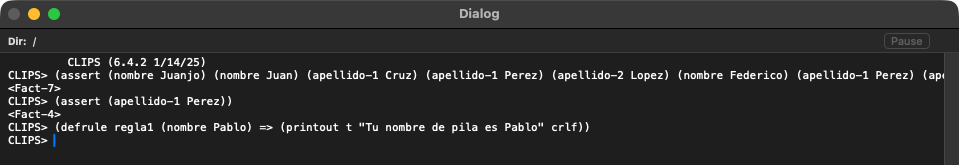
\includegraphics[width=0.75\linewidth]{1_1_dialog_rec.png}
\end{figure}

\subsection{Cuestiones 1.2}

\begin{lstlisting}
(defrule regla1 (nombre Pablo) => (printout t "Tu nombre de pila es Pablo" crlf))
(defrule regla2 (nombre Pablo) (apellido-1 Pardo) (apellido-2 Cotos)
   => (printout t "Te llamas Pablo Pardo Cotos" crlf))
\end{lstlisting}

\textbf{¿Se ha activado alguna regla? ¿Qué hechos activan cada regla?}

Con los hechos del ejercicio 1.1 no se activa ninguna, porque ninguno encaja con sus antecedentes. Al añadir \texttt{(nombre Pablo)}, \texttt{(apellido-1 Pardo)} y \texttt{(apellido-2 Cotos)} (f-8, f-9 y f-10) se activan las dos:

\begin{itemize}
\item \texttt{regla1}, con f-8.
\item \texttt{regla2}, con f-8, f-9 y f-10.
\end{itemize}

\begin{figure}[H]
\centering
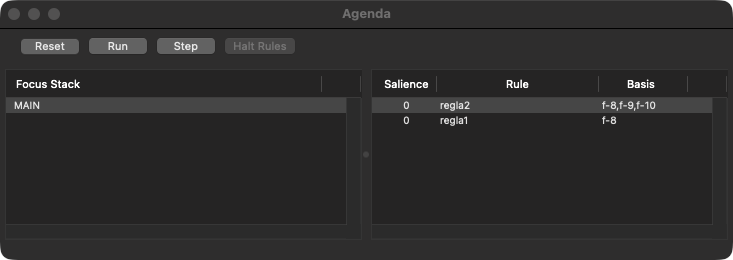
\includegraphics[width=0.65\linewidth]{1_2_agenda.png}
\end{figure}

\subsection{Cuestiones 1.3}

\textbf{¿Qué regla se ejecuta en primer lugar? ¿Por qué?}

\texttt{regla2}. Las dos reglas están en la Agenda, que es el conjunto conflicto, y el motor de inferencia selecciona cuál aplicar. Las dos tienen saliencia 0, y \texttt{regla2}, que fue la última en activarse al añadirse f-10, aparece la primera en la Agenda y es la que se ejecuta.

\begin{figure}[H]
\centering
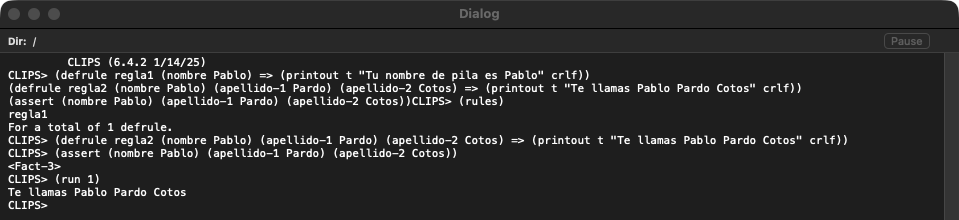
\includegraphics[width=0.75\linewidth]{1_3_run1_dialog_rec.png}
\end{figure}

\textbf{¿Qué pasa si reiniciamos con (clear)?}

Se borran la BH, las reglas y la Agenda. Después de \texttt{(clear)}, \texttt{(facts)} y \texttt{(rules)} no muestran nada.

\begin{figure}[H]
\centering
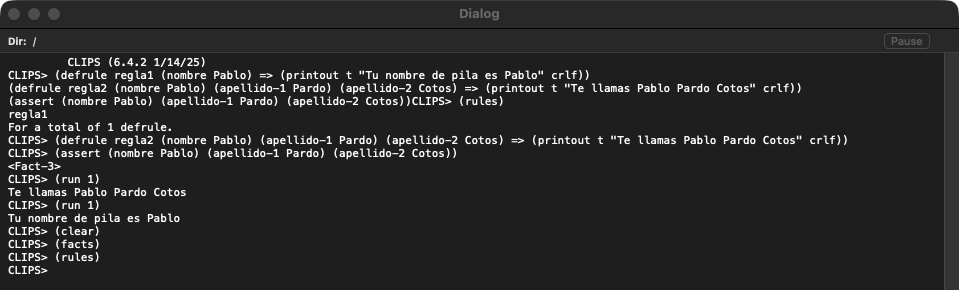
\includegraphics[width=0.75\linewidth]{1_3_clear_dialog_rec.png}
\end{figure}

\subsection{Cuestiones 1.4}

Los hechos se definieron con \texttt{deffacts} en \texttt{1\_4\_hechos\_y\_reglas.clp}, junto con las dos reglas.

\textbf{Si se introducen los hechos con (deffacts) y se carga el fichero, ¿qué ocurre en la BH y en la Agenda?}

No ocurre nada y las dos siguen vacías, porque cargar un \texttt{deffacts} solo define los hechos iniciales, pero no los añade a la BH.

\textbf{¿Qué ocurre en la BH y en la Agenda al ejecutar (reset)?}

Se vacían la BH y la Agenda y se afirman los hechos del \texttt{deffacts}. Entran 10 hechos, porque el duplicado se descarta, y se activan \texttt{regla2} y \texttt{regla1}. Al ejecutar, el resultado es el mismo que en el ejercicio anterior.

\textbf{¿Cuál es el primer hecho que se ha almacenado en la BH?}

\texttt{f-1 (nombre Juanjo)}, el primero del \texttt{deffacts}.

\begin{figure}[H]
\centering
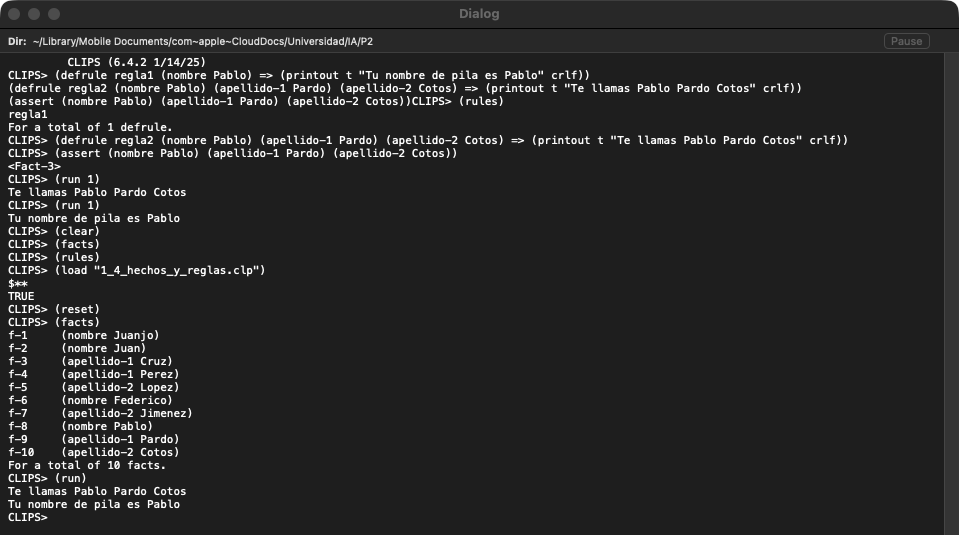
\includegraphics[width=0.75\linewidth]{1_4_run_dialog_rec.png}
\end{figure}

\subsection{Cuestiones 1.5}

Programa \texttt{1\_5\_semaforo.clp}:

\begin{lstlisting}
(defrule regla-tipo-agente
   =>
   (printout t "Que tipo de agente es (vehiculo/peaton)? ")
   (assert (tipo-agente (read))))

(defrule regla-semaforo-vehiculo
   (tipo-agente vehiculo)
   =>
   (printout t "Como esta el semaforo para los coches (verde/rojo/ambar/intermitente)? ")
   (assert (semaforo (read))))

(defrule regla-semaforo-peaton
   (tipo-agente peaton)
   =>
   (printout t "Como esta el semaforo para los peatones (verde/rojo/ambar/intermitente)? ")
   (assert (semaforo (read))))

(defrule agente-puede-pasar
   (tipo-agente ?tipo) (semaforo verde)
   =>
   (printout t "El agente " ?tipo " puede pasar" crlf))

(defrule debe-esperar
   (tipo-agente ?tipo) (semaforo rojo)
   =>
   (printout t "El agente " ?tipo " debe esperar" crlf))

(defrule con-cuidado
   (tipo-agente ?tipo) (semaforo ambar | intermitente)
   =>
   (printout t "El agente " ?tipo " debe pasar con cuidado" crlf))
\end{lstlisting}

\textbf{¿Qué devuelve el programa cuando el agente es un coche y el semáforo para los coches está en rojo?}

\begin{lstlisting}
CLIPS> (load "1_5_semaforo.clp")
******
TRUE
CLIPS> (reset)
CLIPS> (run)
Que tipo de agente es (vehiculo/peaton)? vehiculo
Como esta el semaforo para los coches (verde/rojo/ambar/intermitente)? rojo
El agente vehiculo debe esperar
\end{lstlisting}

\textbf{Errores de compilación provocados}

\begin{center}
\small
\begin{tabularx}{\linewidth}{@{}>{\raggedright\arraybackslash}p{0.36\linewidth}Y@{}}
\toprule
Error introducido & Mensaje de CLIPS \\
\midrule
Quitar un paréntesis & \texttt{[PRNTUTIL2] Syntax Error: Check appropriate syntax for defrule.} \\
\texttt{assertgdf} en lugar de \texttt{assert} & \texttt{[EXPRNPSR3] Missing function declaration for 'assertgdf'.} \\
\texttt{defruledg} en lugar de \texttt{defrule} & \texttt{[EXPRNPSR3] Missing function declaration for 'defruledg'.} \\
Suprimir el nombre de la regla & \texttt{[CSTRCPSR2] Missing name for defrule construct.} \\
\texttt{Printout} o \texttt{DEFRULE} en mayúsculas & \texttt{[EXPRNPSR3] Missing function declaration for 'Printout'.} \\
Quitar el \texttt{;} de un comentario & \texttt{[CSTRCPSR1] Expected the beginning of a construct.} \\
Variable del consecuente no definida en el antecedente & \texttt{[PRCCODE3] Undefined variable ?tipo referenced in RHS of defrule.} \\
\texttt{->} en lugar de \texttt{=>} & \texttt{[PRNTUTIL2] Syntax Error: Check appropriate syntax for defrule.} \\
\bottomrule
\end{tabularx}
\end{center}
